\section{Photonik Aktoren}
\subsection{Lichtquellen}
\subsubsection{Temperaturstrahler}
\begin{multicols}{2}
    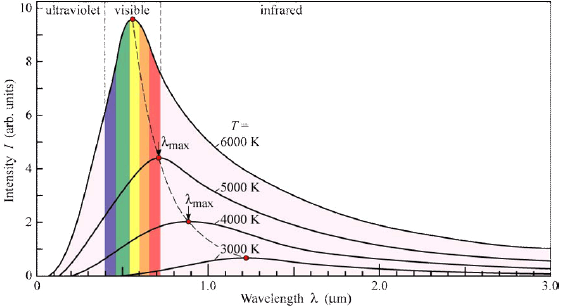
\includegraphics[width=0.5\textwidth]{images/temperaturstrahler} \vfill \columnbreak
    Die Temperaturstrahler können in zwei kategorien eingeteilt werden:
    \begin{compactitem}
        \item Natürliche Temperaturstrahler: Sterne, Blitze, Feuer, ...
        \item Künstliche Temperaturstrahler: Kerzen, Glühbirnen, ... 
    \end{compactitem}
    Jeder Körper mit Temperatur wärmer als der absolute Nullpunkt gibt elektromagnetische Strahlung ab.
    Die Temperatur bestimmt dabei die Lichtintensität: $I=\sigma*T^4$
\end{multicols}

\subsection{Die Sonne}
\subsubsection{Sonneneinstrahlung}
Der Bezugswert der Sonneneinstrahlung für die Erde ist mit der Solarkonstante festgelegt. Sie hat den Wert $1.37 \frac{kW}{m^2}$ für senkrecht zur Probefläche einfallendes Licht ohne atmosphärische Einflüsse, also ausserhalb der Atmosphäre. Dieser Wert gilt damit für die Verhältnisse im Weltraum. Bei unbedecktem Himmel, trockener Luft und am Erdboden ist der Wert der sogenannten terrestrischen Solarkonstante $1 \frac{kW}{m^2}$. Als Vergleich zur Stärke der Sonneneinstrahlung kann man eine kleine Herdplatte heranziehen. Ihre Leistung liegt - auf höchster Stufe - bei etwa einem Kilowatt, ihre Fläche (18cm Durchmesser) bei etwa 0.025m, die Leistung pro Fläche $40 \frac{kW}{m^2}$.

\subsubsection{Airmass AM}
Das Airmass ist ein Mass dafür, wie lang der Weg des Lichts durch die Atmosphäre ist.

\subsection{Glühlampe}
In einer Glühlampe fliesst ein elektrischer Strom durch einen dünnen Leiter, z.B. ein Metall-Faden aus Wolfram. Fliesst ein ausreichend starker elektrischer Strom wird dieser erhitzt, so dass er glüht. Die Temperatur der Glühwendel beträgt je nach Bauform ca. $1500$ – $3000^\degree C$, so dass sie gemäss dem planckschen Strahlungsgesetz elektromagnetische Strahlung emittiert. Die Strahlung liegt vor allem im Bereich der Infrarotstrahlung und nur wenig (\textless5\%) im Bereich des sichtbaren Lichts.

\subsection{Lumineszenz-Strahler}
Unterbegriffe der Lumineszenz sind Fluoreszenz (kurzes Nachleuchten) und Phosphoreszenz (langes Nachleuchten). Es gibt auch hier zwei Varianten:
\begin{compactitem}
    \item Biologische Lumineszenz-Strahler sind Glühwürmchen
    \item Chemische Lumineszenz-Strahler sind z.B. Leuchtstäbe
\end{compactitem}
Strahlung kann abgegeben werden (Lumineszenz) oder aufgenommen werden (Photoeffekt) nach dem Gesetz: $\Delta E = h*v$ wobei $h = 6.6*10^{-34} \frac{J}{Hz}$

\subsection{Leuchtdioden (Light Emitting Diode)}
\subsubsection{Funktionsweise}
\begin{wrapfigure}{r}{0.25\textwidth}
    \centering
    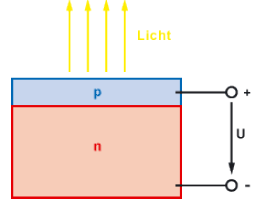
\includegraphics[width=0.22\textwidth]{images/LED}
\end{wrapfigure}
Eine Leuchtdiode besteht aus einem n-leitenden Grundhalbleiter. Darauf ist eine sehr dünne p-leitende Halbleiterschicht mit grosser Löcherdichte aufgebracht. Wie bei der normalen Diode wird die Grenzschicht mit freien Ladungsträgern überschwemmt. Die Elektronen rekombinieren mit den Löchern. Dabei geben die Elektronen ihre Energie in Form eines Lichtblitzes frei. Da die p-Schicht sehr dünn ist, kann das Licht entweichen. Da von dem Halbleiterkristall nur eine geringe Lichtstrahlung ausgeht, ist das Metall unter dem Kristall halbkugelförmig. Dadurch wird das Licht gestreut. Durch das linsenförmige Gehäuse wird das Licht gebündelt. So können Leuchtdioden schon mit wenigen milliampere Strom sehr hell leuchten.

\subsubsection{Farben und Materialien}
\begin{wrapfigure}[4]{l}{0.5\textwidth}
    \vspace{-12pt}
    \centering
    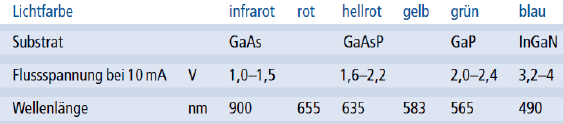
\includegraphics[width=0.48\textwidth]{images/kennwert_LED}
\end{wrapfigure}
Die Farbe des Lichts bzw. die Wellenlänge des Lichts wird vom Halbleiterkristall und von der Dotierung bestimmt. \\

\subsection{Laser (Light Amplification by Stimulated Emission of Radiation)}
\begin{wrapfigure}[7]{l}{0.5\textwidth}
    \vspace{-12pt}
    \centering
    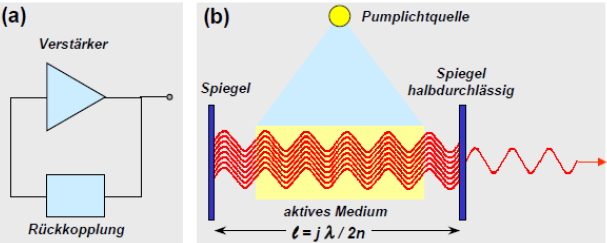
\includegraphics[width=0.48\textwidth]{images/laser}
\end{wrapfigure}
Der Laser ist eine monochrome, kohärente, polarisierte Lichtquelle mit hoher Intensität und scharfer Bündelung des Strahls. Es gibt dabei drei verschiedene Arten: Gas-, Farbstoff-, Halbleiterlaser.

\subsubsection{Funktionsweise}
Der Laser ist ein Resonator zwischen 2 Spiegeln, das Licht tritt an halbdurchlässigem Spiegel aus.

\subsubsection{Laserdiode}
\begin{wrapfigure}[4]{l}{0.25\textwidth}
    \vspace{-12pt}
    \centering
    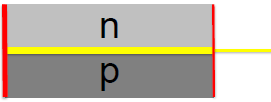
\includegraphics[width=0.22\textwidth]{images/laserdiode}
\end{wrapfigure}
Die Laserdiode hat pn-Übergang und zwei spiegelnde Flächen. Es erfolgt eine stimulierte Emission (bei LED spontane Emission). Ein einfallendes Photon regt dabei ein zweites Photon an. Dieses besitzt exakt dieselben Eigenschaften (Wellenlänge, Ausbreitungsrichtung und Polarisation). Erst ab Schwellstrom ($I_{th}$)funktioniert die Diode als Laser, sonst ist es nur eine LED! Die Laserdioden werden auf Wafern hergestellt. Die Wafer werden geschnitten. Danach müssen die Schnittflächen verspiegelt werden. 

\subsubsection{Laserdiode VCSEL}
\begin{wrapfigure}[6]{l}{0.25\textwidth}
    \vspace{-12pt}
    \centering
    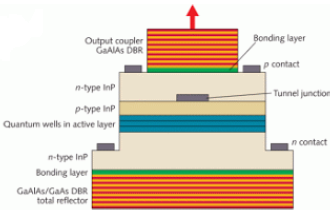
\includegraphics[width=0.22\textwidth]{images/vcsel}
\end{wrapfigure}
Bei VCSEL (Vertical Cavity Surface Emitting Laser) werden die spiegelnden Flächen auf dem Wafer abgeschieden. Viele Schichten aus Materialien mit unterschiedlichem Brechungsindex ergeben dabei einen Interferenzfilter, welcher die gewünschte Wellenlänge spiegelt. Der Aufbau ist komplex, aber es lassen sich zehntausende Laser auf einem Wafer gleichzeitig herstellen. VCSEL sind somit deutlich billiger als normale Laserdioden.




